\chapter{THIẾT KẾ VÀ THỰC HIỆN PHẦN MỀM NHÚNG CHO HIL}
\section{Yêu cầu thiết kế}
Các yêu cầu thiết kế chính cho phần mềm nhúng trên hệ thống mô phỏng phần cứng trong HIL bao gồm:
\begin{itemize}
    \item HIL phải có khả năng giao tiếp USB với máy tính để nhận lệnh cấu hình và điều khiển mô phỏng.
    \item HIL phải có khả năng giao tiếp với DUT thông qua các giao thức ngoại vi phổ biến như UART, I2C, SPI,...
    \item Hệ thống HIL cần mô phỏng chính xác hành vi của các thiết bị ngoại vi, bao gồm việc tạo và xử lý tín hiệu đầu vào/đầu ra theo thời gian thực hoặc gần thời gian thực.
    \item Phần mềm nhúng trên hệ thống HIL phải có khả năng cấu hình linh hoạt các tham số giao tiếp như tốc độ truyền nhận, địa chỉ I2C, định dạng dữ liệu,...
    \item Hệ thống HIL cần hỗ trợ việc ghi nhận và phân tích dữ liệu giao tiếp để phục vụ mục đích debug và đánh giá hiệu suất của DUT.
\end{itemize}

\section{Lưu đồ giải thuật tổng quát của hệ thống HIL}

Lưu đồ giải thuật tổng quát mô tả trình tự hoạt động chính của hệ thống HIL được trình bày trong Hình \ref{fig:HIL_overview}.

\begin{figure}[H]
    \centering
    
\includegraphics[width=0.3\textwidth]{image/HIL_overview.jpg}
    \caption{Lưu đồ giải thuật tổng quát của hệ thống HIL}
    \label{fig:HIL_overview}
\end{figure}

Quá trình hoạt động của hệ thống HIL bắt đầu bằng giai đoạn khởi tạo. Trong giai đoạn này, vi điều khiển thực hiện cấu hình xung clock hệ thống và khởi tạo các ngoại vi cần thiết như USB, UART, I2C, SPI và các bộ định thời. Việc khởi tạo này đảm bảo các tài nguyên phần cứng sẵn sàng cho quá trình mô phỏng và giao tiếp.

Sau khi hoàn tất khởi tạo, hệ thống tiến hành tạo các task phục vụ cho việc xử lý lệnh từ máy tính và mô phỏng thiết bị ngoại vi. Trong suốt quá trình vận hành, hệ thống HIL liên tục nhận các lệnh cấu hình và điều khiển mô phỏng từ máy tính, sau đó thực hiện các hành vi mô phỏng tương ứng và gửi tín hiệu đến DUT.

Khi DUT phản hồi dữ liệu thông qua các giao thức ngoại vi, hệ thống HIL tiến hành thu thập, xử lý và cập nhật trạng thái mô phỏng. Chu trình này được lặp lại liên tục, đảm bảo hệ thống HIL hoạt động ổn định và đáp ứng kịp thời các yêu cầu kiểm thử firmware.

\section{Lưu đồ giải thuật chi tiết của task xử lý lệnh}

Để đảm bảo khả năng điều khiển linh hoạt từ máy tính, hệ thống HIL triển khai một task chuyên trách cho việc xử lý lệnh. Lưu đồ giải thuật của task này được minh họa trong Hình \ref{fig:HIL_CLI_task}.

\begin{figure}[H]
    \centering
    
\includegraphics[width=0.7\textwidth]{image/HIL_CLI_task.jpg}
    \caption{Lưu đồ giải thuật của task xử lý lệnh từ máy tính}
    \label{fig:HIL_CLI_task}
\end{figure}

Task xử lý lệnh hoạt động theo cơ chế vòng lặp vô hạn, liên tục chờ dữ liệu từ máy tính thông qua giao tiếp USB. Khi nhận được một lệnh, hệ thống tiến hành phân tích cú pháp và xác định loại lệnh tương ứng.

Đối với các lệnh cấu hình, hệ thống HIL cập nhật các tham số liên quan đến giao tiếp và mô phỏng, bao gồm tốc độ truyền, địa chỉ thiết bị, chế độ hoạt động và định dạng dữ liệu. Các thay đổi này được áp dụng ngay lập tức mà không cần khởi động lại hệ thống.

Trong trường hợp nhận được lệnh điều khiển mô phỏng, hệ thống sẽ kích hoạt mô hình thiết bị ngoại vi tương ứng và thực hiện các thao tác mô phỏng cần thiết để trao đổi dữ liệu với DUT. Nếu lệnh không hợp lệ hoặc không được hỗ trợ, hệ thống gửi thông báo lỗi về máy tính để người dùng xử lý.

Cơ chế này giúp hệ thống HIL luôn sẵn sàng đáp ứng các yêu cầu kiểm thử và nếu cần có thể mở rộng thêm các loại lệnh trong tương lai.

\section{Lưu đồ giải thuật chi tiết mô phỏng thiết bị ngoại vi}
\subsection{Mô phỏng thiết bị ngoại vi giao tiếp I2C}

Hệ thống HIL hỗ trợ mô phỏng các thiết bị ngoại vi giao tiếp I2C nhằm phục vụ kiểm thử firmware của DUT. Trong phạm vi đề tài, hai thiết bị I2C được lựa chọn để mô phỏng là EEPROM và RTC, do đây là các thiết bị phổ biến trong nhiều hệ thống nhúng.

Quy trình mô phỏng thiết bị I2C trong hệ thống HIL được trình bày trong Hình \ref{fig:I2C_device}.

\begin{figure}[H]
    \centering
    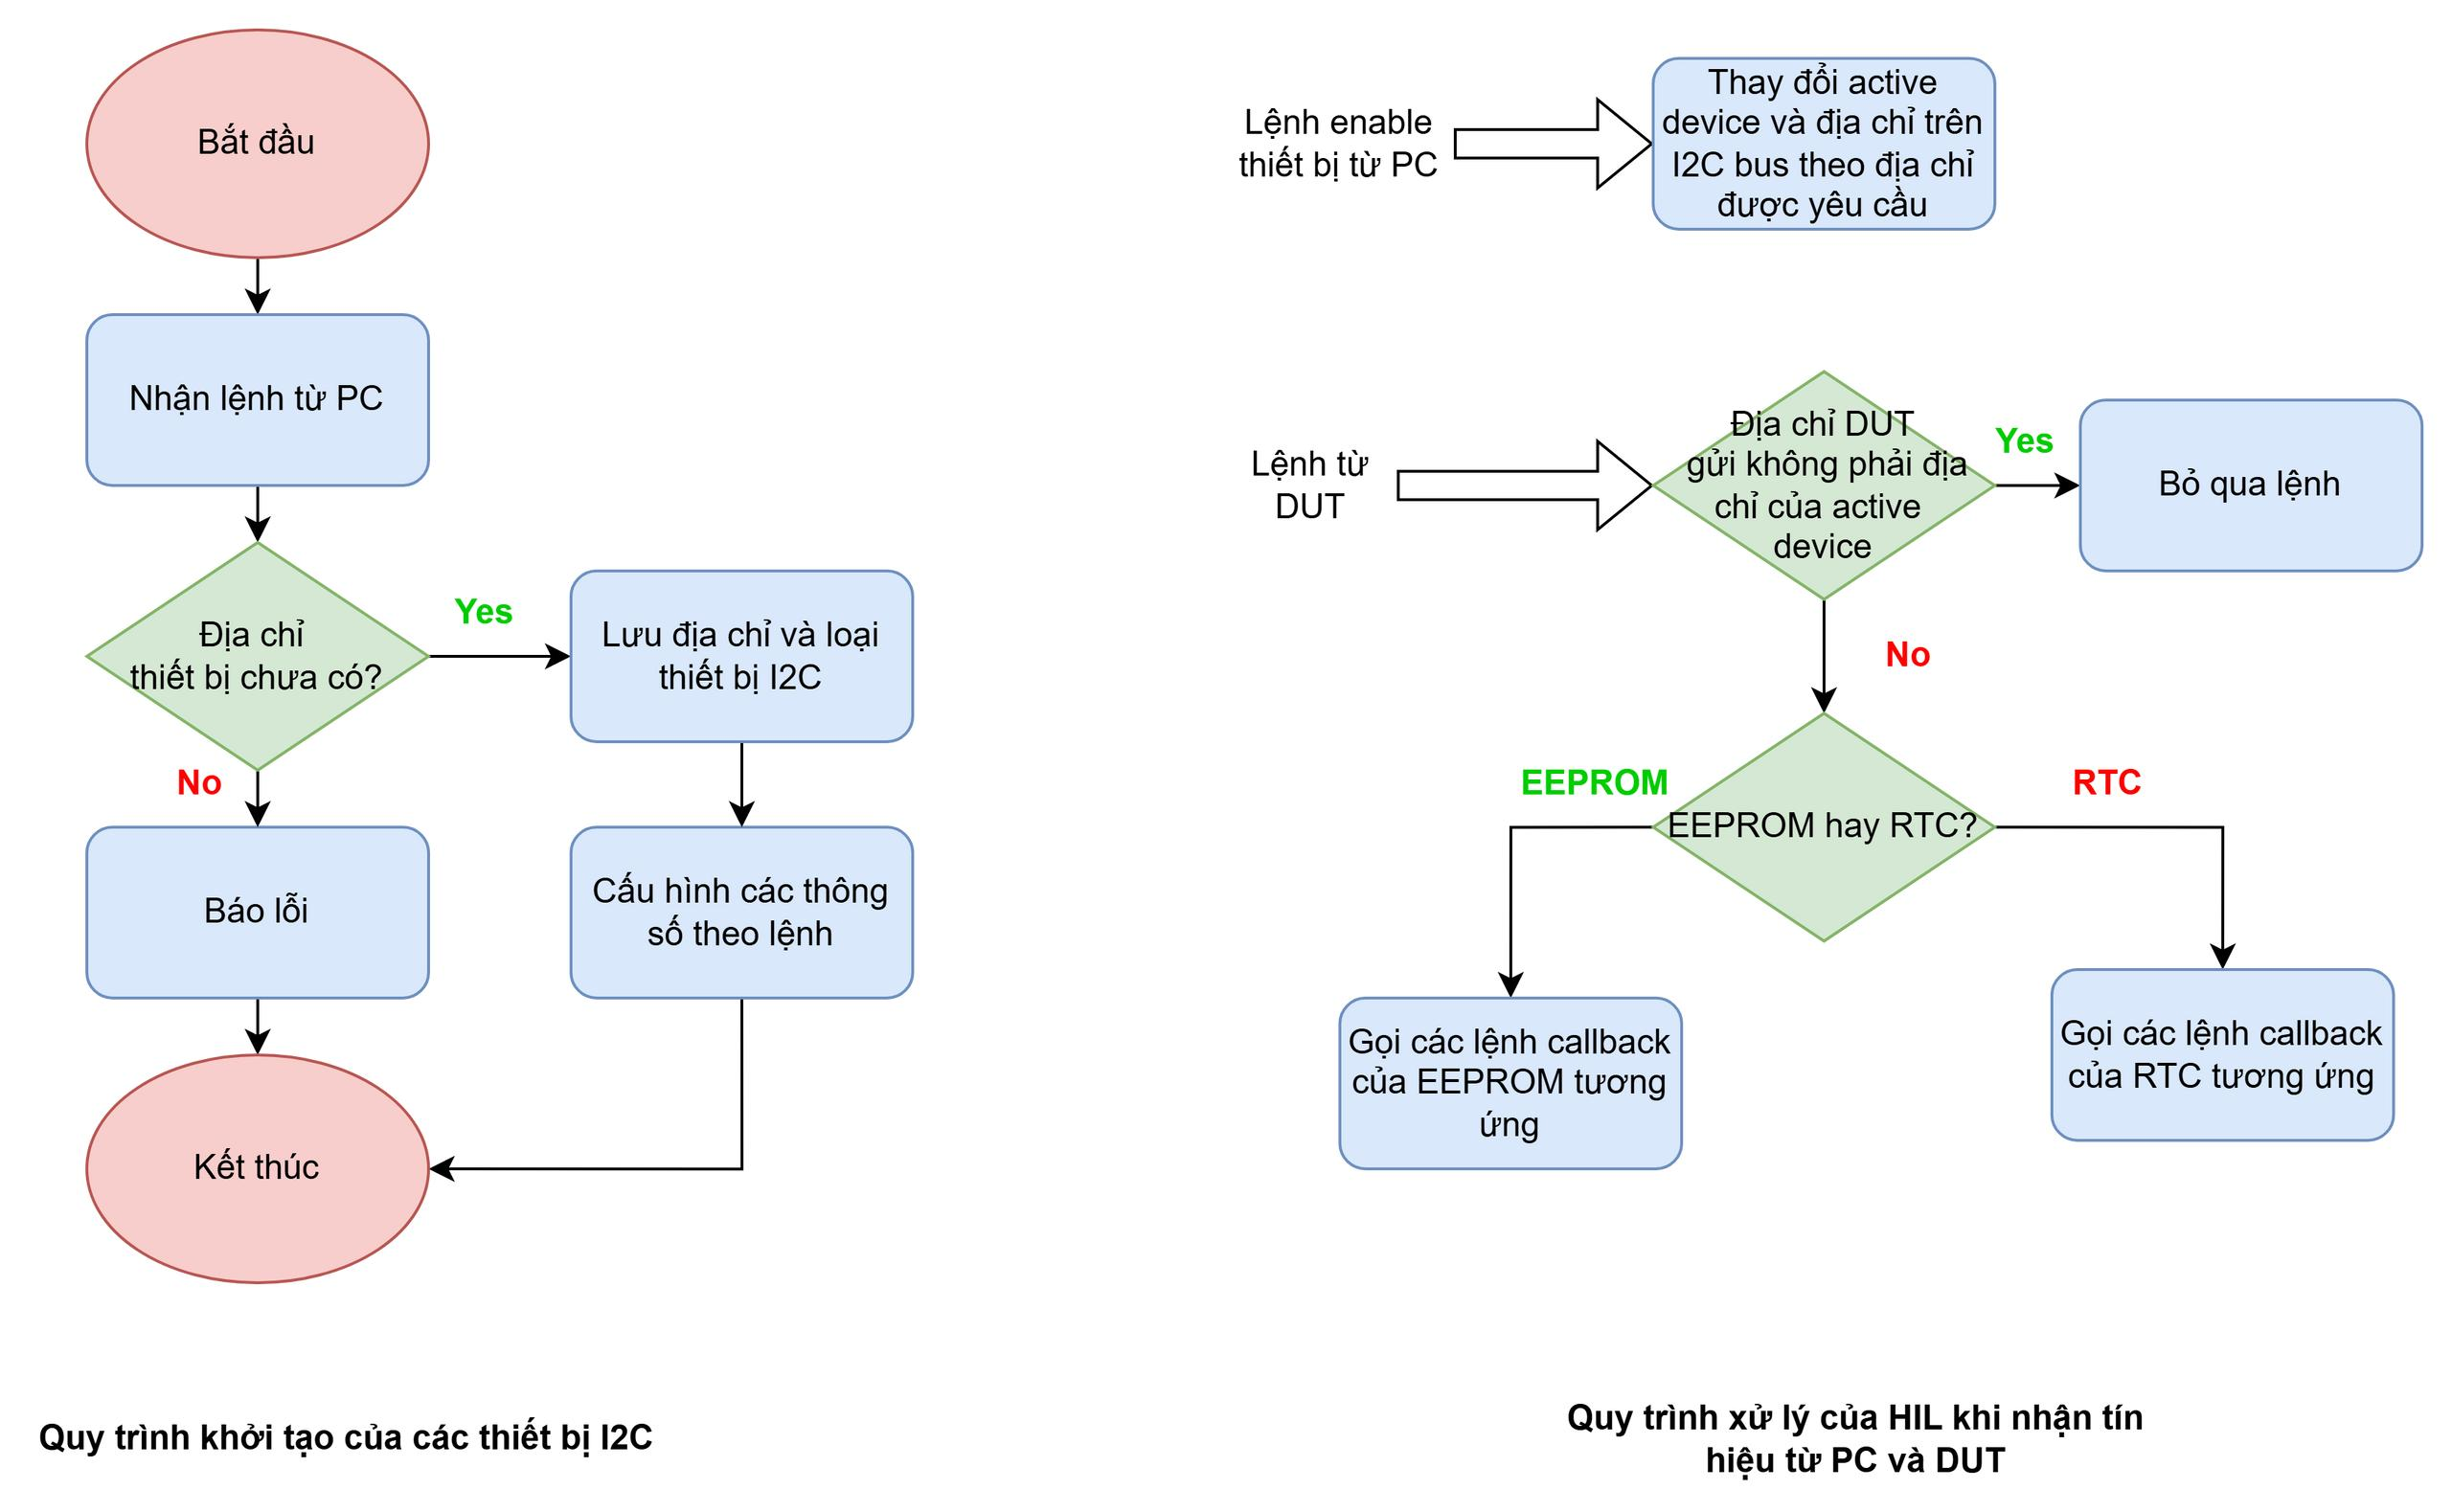
\includegraphics[width=1\textwidth]{image/I2C_device.png}
    \caption{Quy trình mô phỏng thiết bị I2C trong hệ thống HIL}
    \label{fig:I2C_device}
\end{figure}

Để khởi tạo một thiết bị I2C mô phỏng, hệ thống HIL cần nhận lệnh cấu hình từ máy tính, bao gồm loại thiết bị và địa chỉ I2C tương ứng. Do số lượng địa chỉ I2C phần cứng trên vi điều khiển bị giới hạn, các thiết bị I2C trong hệ thống HIL được quản lý hoàn toàn ở mức phần mềm.

Khi nhận được yêu cầu khởi tạo, hệ thống kiểm tra xem địa chỉ I2C đã được sử dụng hay chưa. Nếu địa chỉ đã tồn tại trong danh sách quản lý, hệ thống từ chối khởi tạo và gửi thông báo lỗi về máy tính. Ngược lại, nếu địa chỉ hợp lệ, thiết bị mô phỏng được khởi tạo và lưu vào danh sách quản lý thiết bị I2C.

Trong quá trình DUT giao tiếp trên bus I2C, hệ thống HIL giám sát địa chỉ truy cập và kích hoạt mô hình thiết bị tương ứng. Dữ liệu phản hồi được tạo ra dựa trên mô hình hành vi của thiết bị, đảm bảo tính tương đương với thiết bị thực.

Đối với thiết bị EEPROM, hệ thống HIL mô phỏng bộ nhớ lưu trữ theo từng trang, trong đó dữ liệu ghi từ DUT được đệm tạm và chỉ được ghi chính thức vào vùng nhớ mô phỏng khi phiên giao tiếp I2C kết thúc. Cách tiếp cận này đảm bảo hành vi ghi dữ liệu tương đương với EEPROM thực, bao gồm cơ chế tự tăng địa chỉ và giới hạn kích thước trang.

Đối với thiết bị RTC, hệ thống HIL mô phỏng tập thanh ghi thời gian theo chuẩn của DS1307 và sử dụng bộ định thời nội để cập nhật giá trị thời gian thực theo chu kỳ 1 giây. DUT có thể thực hiện các thao tác đọc và ghi để lấy hoặc thiết lập thời gian, trong đó dữ liệu được mã hóa theo định dạng BCD giống với thiết bị phần cứng thực tế.

\subsection{Mô phỏng thiết bị ngoại vi giao tiếp SPI}

Bên cạnh giao tiếp I2C, hệ thống HIL còn hỗ trợ mô phỏng các thiết bị ngoại vi sử dụng giao thức SPI nhằm kiểm thử các chức năng firmware của DUT liên quan đến bộ nhớ ngoài. Trong phạm vi đề tài, thiết bị SPI được lựa chọn để mô phỏng là bộ nhớ Flash W25Q, một linh kiện phổ biến trong các hệ thống nhúng dùng để lưu trữ chương trình và dữ liệu.

Thiết bị Flash SPI được mô phỏng theo mô hình slave, trong đó hệ thống HIL đóng vai trò phản hồi các lệnh truy cập từ DUT thông qua bus SPI. Toàn bộ nội dung bộ nhớ Flash được mô phỏng bằng vùng nhớ RAM trong vi điều khiển của HIL, cho phép truy cập nhanh và linh hoạt trong quá trình kiểm thử.

Quy trình mô phỏng thiết bị SPI trong hệ thống HIL được trình bày trong Hình~\ref{fig:SPI_flash}.

\begin{figure}[H]
    \centering
    
\includegraphics[width=0.35\textwidth]{image/SPI_flash.png}
    \caption{Quy trình mô phỏng bộ nhớ SPI flash trong hệ thống HIL}
    \label{fig:SPI_flash}
\end{figure}

Quá trình mô phỏng SPI bắt đầu khi DUT kích hoạt tín hiệu Chip Select (NSS) ở mức thấp, báo hiệu một phiên giao tiếp SPI mới. Hệ thống HIL sử dụng ngắt ngoài để phát hiện sự kiện này và tiến hành khởi tạo lại các biến trạng thái nội bộ, đảm bảo mỗi transaction SPI được xử lý độc lập và chính xác.

Byte dữ liệu đầu tiên được DUT truyền đến được xem là lệnh điều khiển (opcode). Dựa trên opcode nhận được, hệ thống HIL xác định loại lệnh tương ứng và chuyển sang trạng thái xử lý phù hợp. Trong phạm vi đề tài, các lệnh cơ bản của Flash SPI như đọc ID, đọc dữ liệu, ghi dữ liệu và xóa bộ nhớ được mô phỏng.

Đối với lệnh đọc ID, hệ thống HIL phản hồi lần lượt các byte định danh thiết bị, cho phép DUT xác nhận đúng loại Flash đang được sử dụng. Với lệnh đọc dữ liệu, sau khi nhận đủ địa chỉ truy cập, hệ thống bắt đầu truyền dữ liệu từ bộ nhớ mô phỏng về DUT, đồng thời tự động tăng địa chỉ để mô phỏng cơ chế đọc liên tục của Flash thực.

Trong trường hợp lệnh ghi dữ liệu, hệ thống HIL tiếp nhận dữ liệu từ DUT và lưu vào vùng nhớ mô phỏng tương ứng với địa chỉ đã chỉ định. Đối với lệnh xóa bộ nhớ, toàn bộ vùng nhớ mô phỏng được đưa về trạng thái mặc định, tương đương với quá trình xóa chip của Flash thực tế.

Trong suốt quá trình giao tiếp SPI, hệ thống HIL gửi các byte dummy khi cần thiết nhằm duy trì xung clock và đảm bảo đồng bộ truyền nhận giữa master và slave. Cơ chế này giúp DUT hoạt động bình thường mà không cần thay đổi firmware khi chuyển từ thiết bị Flash thực sang Flash mô phỏng.

Việc mô phỏng thiết bị SPI trong hệ thống HIL cho phép kiểm thử đầy đủ các chức năng liên quan đến bộ nhớ ngoài của DUT mà không cần sử dụng phần cứng Flash thật. Điều này giúp giảm chi phí phần cứng, đồng thời tăng tính linh hoạt và khả năng tự động hóa trong quá trình phát triển và kiểm thử firmware nhúng.

\section{Lưu đồ giải thuật xử lý các ngoại vi}
\subsection{Xử lý UART/CAN}
\begin{figure}[H]
    \centering
    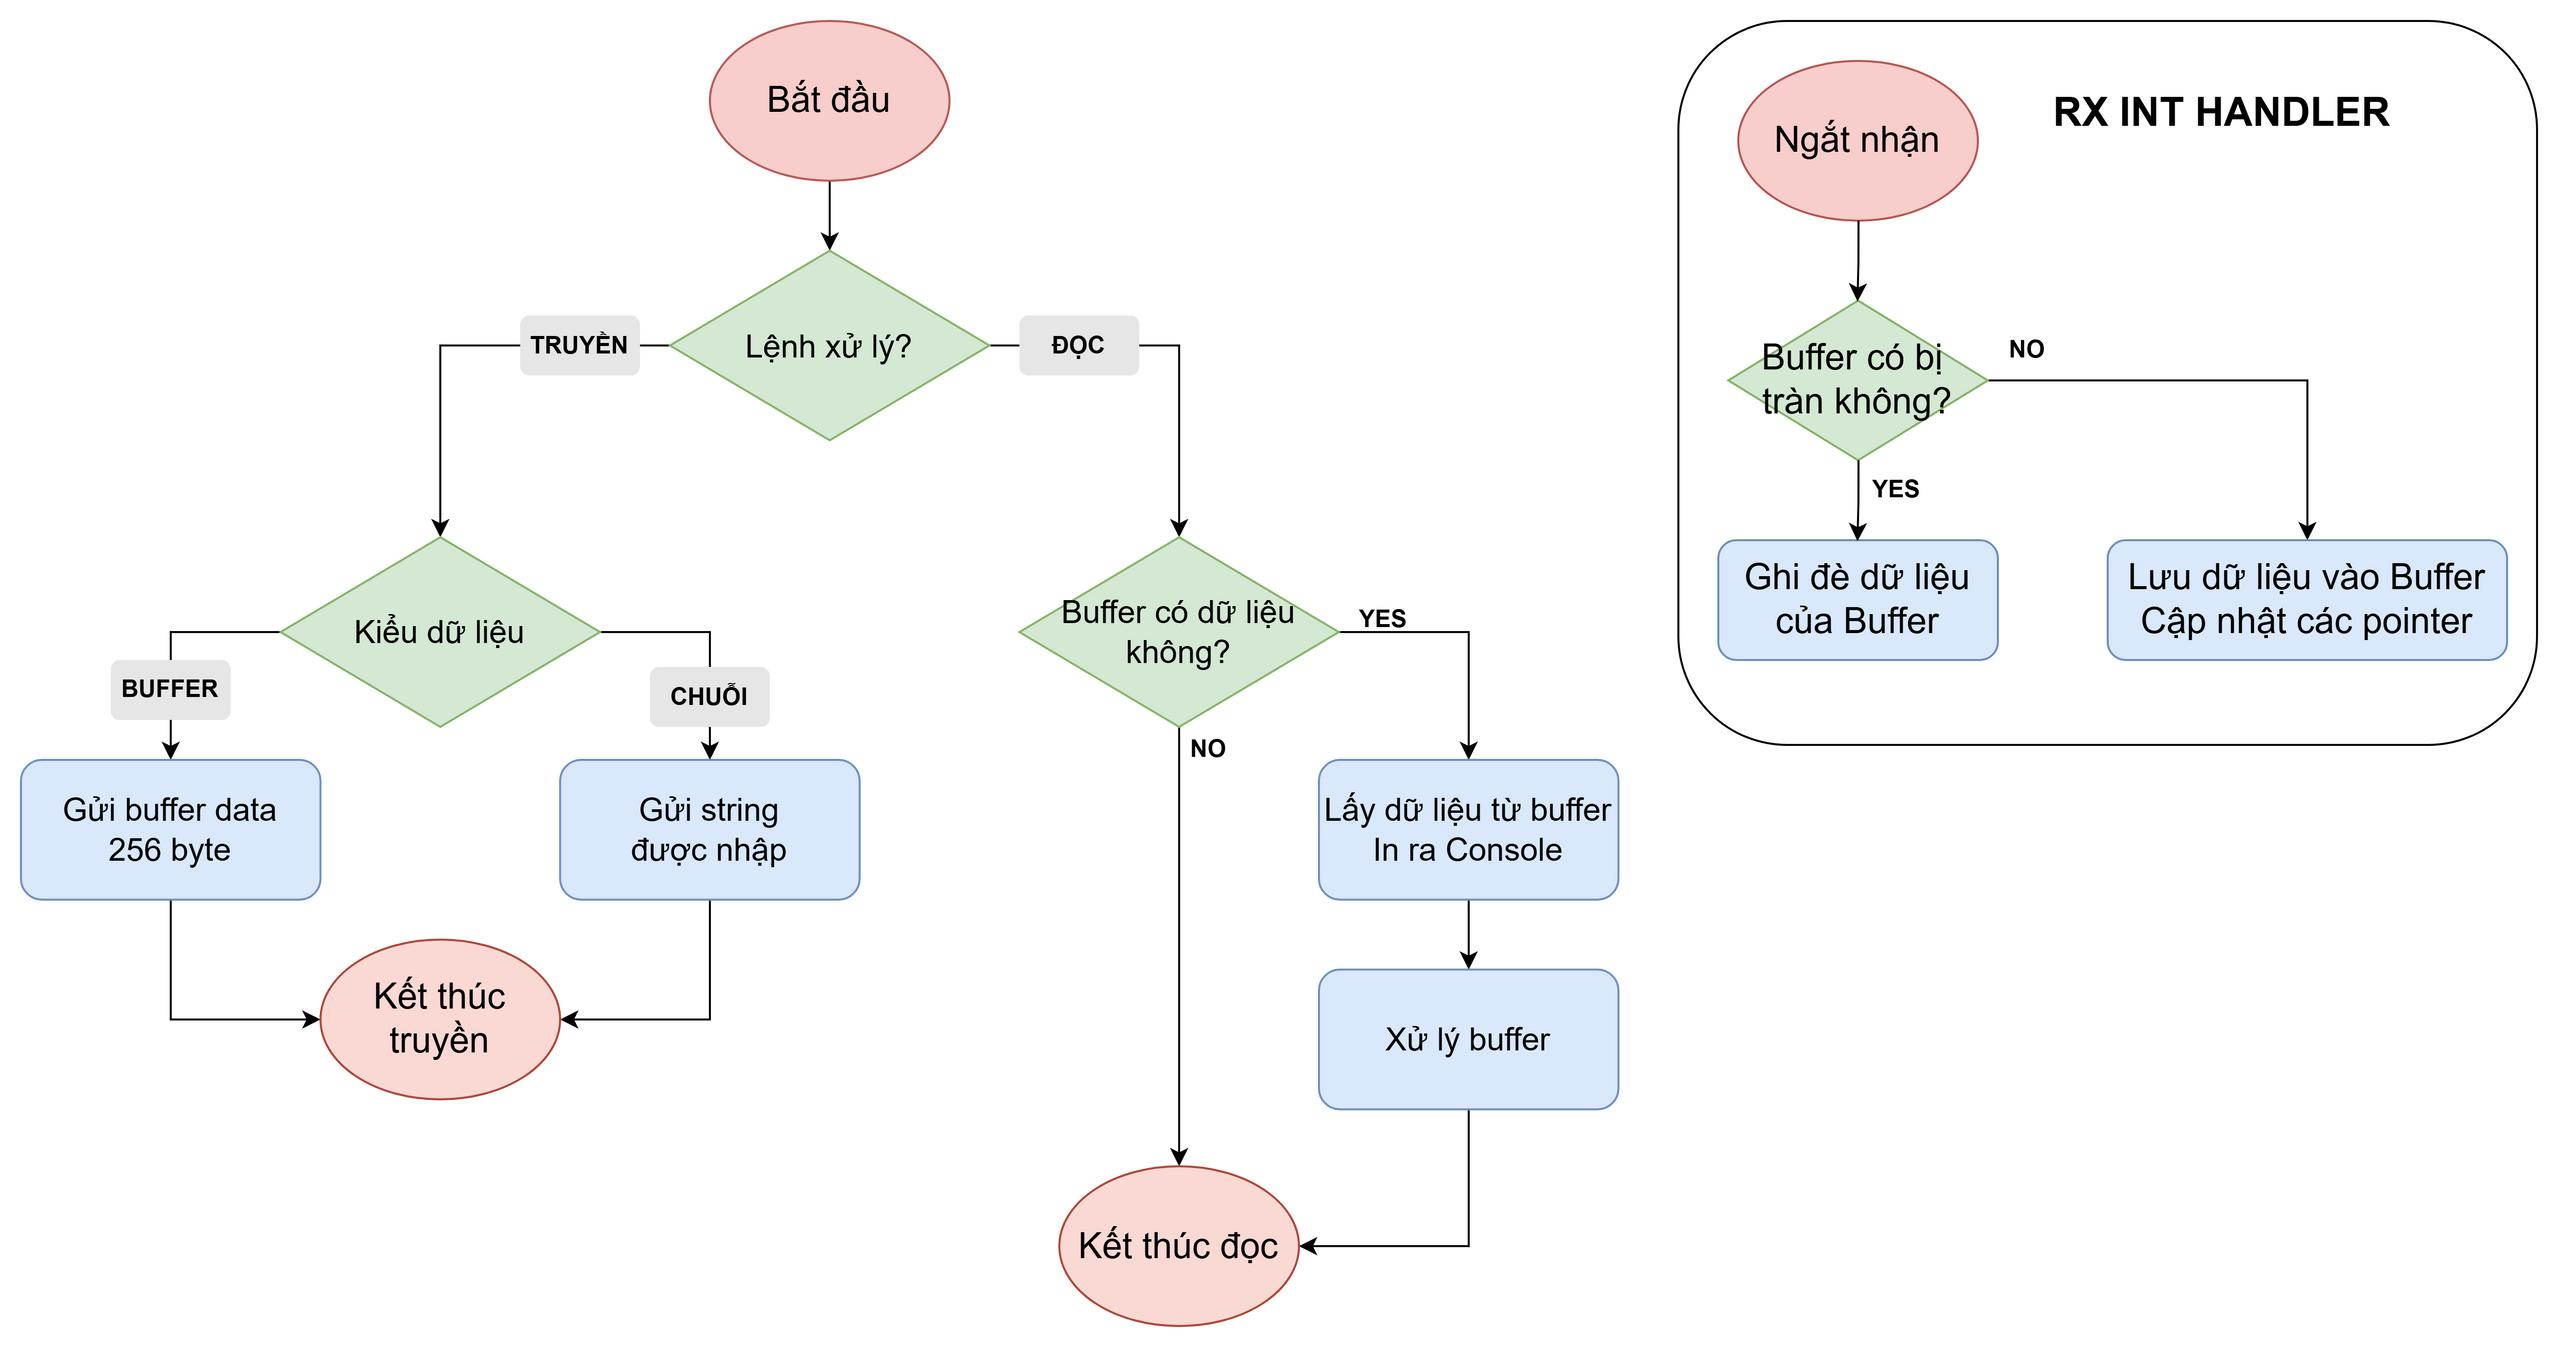
\includegraphics[width=1\textwidth]{image/hil_uart_can.jpg}
    \caption{Lưu đồ giải thuật giao tiếp UART và CAN}
    \label{fig:hil_uart_can}
\end{figure}
Lưu đồ giải thuật trên mô tả quá trình xử lý truyền và nhận dữ liệu của khối giao tiếp UART và CAN trong hệ thống.
Khi hệ thống hoạt động, chương trình sẽ kiểm tra lệnh cần xử lý. Nếu là lệnh truyền dữ liệu, hệ thống sẽ xác định kiểu dữ liệu cần gửi.
Đối với dữ liệu dạng buffer, HIL sẽ gửi toàn bộ khối dữ liệu có kích thước 256 byte thông qua giao thức UART hoặc CAN với các giá trị tăng dần từ 0x00 $\rightarrow$ 0xFF và lặp lại.
Trong trường hợp dữ liệu cần truyền là chuỗi ký tự, hệ thống sẽ gửi chuỗi được nhập đó đến DUT. Sau khi hoàn tất quá trình truyền, hệ thống chuyển sang trạng thái kết thúc truyền và sẵn sàng cho các yêu cầu tiếp theo.

Đối với lệnh truyền dữ liệu, chương trình sẽ kiểm tra trạng thái của buffer nhận để xác định có dữ liệu mới hay không. Nếu buffer chưa có dữ liệu, quá trình đọc sẽ kết thúc.
Nếu buffer đã chứa dữ liệu, chương trình sẽ lấy dữ liệu từ buffer và hiển thị ra console nhằm phục vụ cho mục đích giám sát.
Dữ liệu sẽ được ghi vào buffer trong quá trinh ngắt. Nếu buffer chưa đầy, dữ liệu mới sẽ được lưu vào buffer đồng thời cập nhật các pointer quản lý vị trí đọc và ghi.
Trong trường hợp buffer bị tràn, hệ thống sẽ ghi đè dữ liệu cũ của buffer.

Cơ chế ngắt nhận dữ liệu sẽ được phần cứng tự động kích hoạt mỗi khi có một khung truyền được gửi đến. Tuy nhiên dựa vào Hình \ref{fig:uart_frame} và Hình \ref{fig:can_frame} có thể thấy UART và CAN có khung truyền khác nhau.
Với UART, mỗi khung truyền chỉ có 1 byte dữ liệu nhưng giao thức CAN có thể linh hoạt độ dài của dữ liệu bằng trường DLC cho phép độ dài vùng dữ liệu dao động từ 0 - 8 byte.
Chính vì thế quá trình xử lý ngắt cho UART và CAN được thiết kế với vài điểm khác biệt.
\begin{figure}[H]
    \centering
    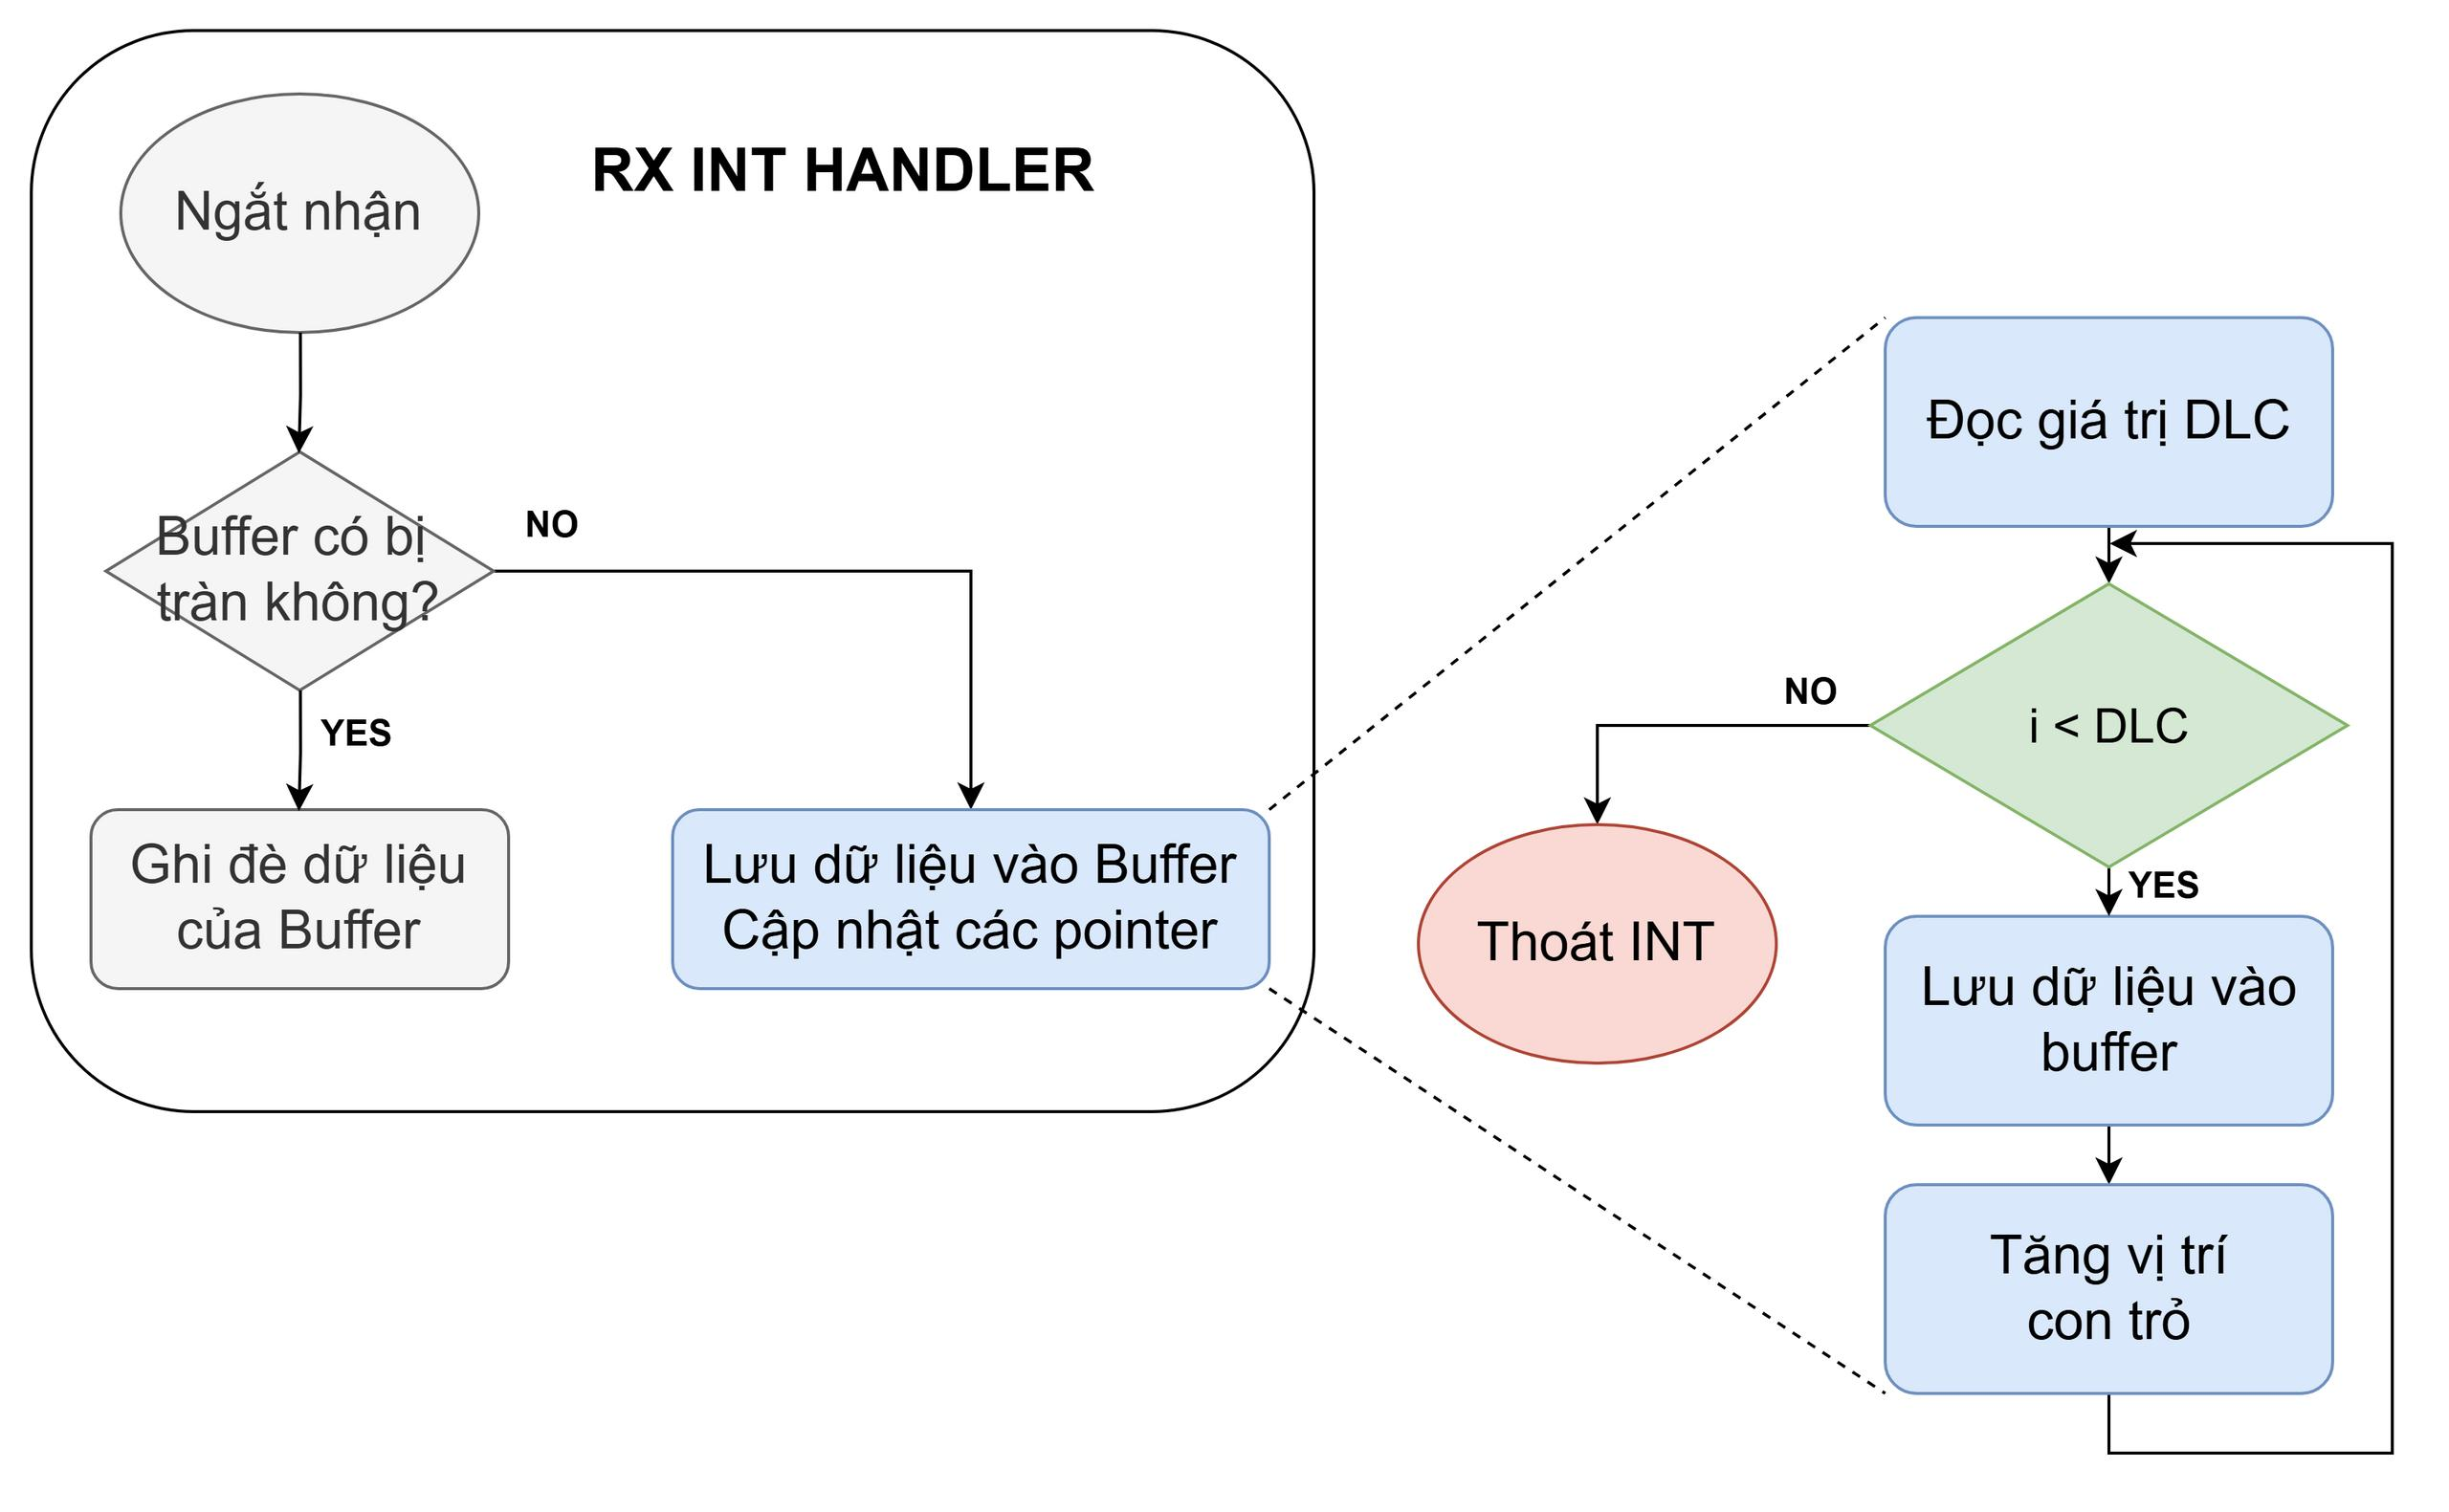
\includegraphics[width=0.65\textwidth]{image/hil_can.jpg}
    \caption{Lưu đồ giải thuật xử lý ngắt nhận của giao thức CAN}
    \label{fig:hil_can}
\end{figure}
Hình \ref{fig:hil_can} mô tả thuật toán xử lý dữ liệu cho giao thức CAN khi có ngắt nhận. Khi một frame CAN được nhận, HIL sẽ trước tiên đọc giá trị từ trường DLC (Data Length Code) để xác định số byte dữ liệu cần xử lý. 
Dựa trên giá trị này, hệ thống thực hiện vòng lặp để lần lượt đọc từng byte dữ liệu và lưu vào buffer. Sau mỗi lần lưu, con trỏ buffer sẽ được tăng lên để chuẩn bị cho vị trí lưu trữ tiếp theo.
Quá trình này tiếp tục cho đến khi toàn bộ số byte tương ứng với giá trị DLC được xử lý hoàn tất, sau đó chương trình sẽ thoát khỏi trình phục vụ ngắt.

Đối với giao tiếp UART, cơ chế xử lý đơn giản hơn do dữ liệu được nhận theo từng byte riêng lẻ. Mỗi khi xảy ra ngắt nhận, hệ thống sẽ đọc một byte dữ liệu và lưu trực tiếp vào buffer. Sau đó, con trỏ buffer được tăng lên để chuẩn bị cho lần nhận tiếp theo.

\subsection{Xử lý ADC/DAC}
\begin{figure}[H]
    \centering
    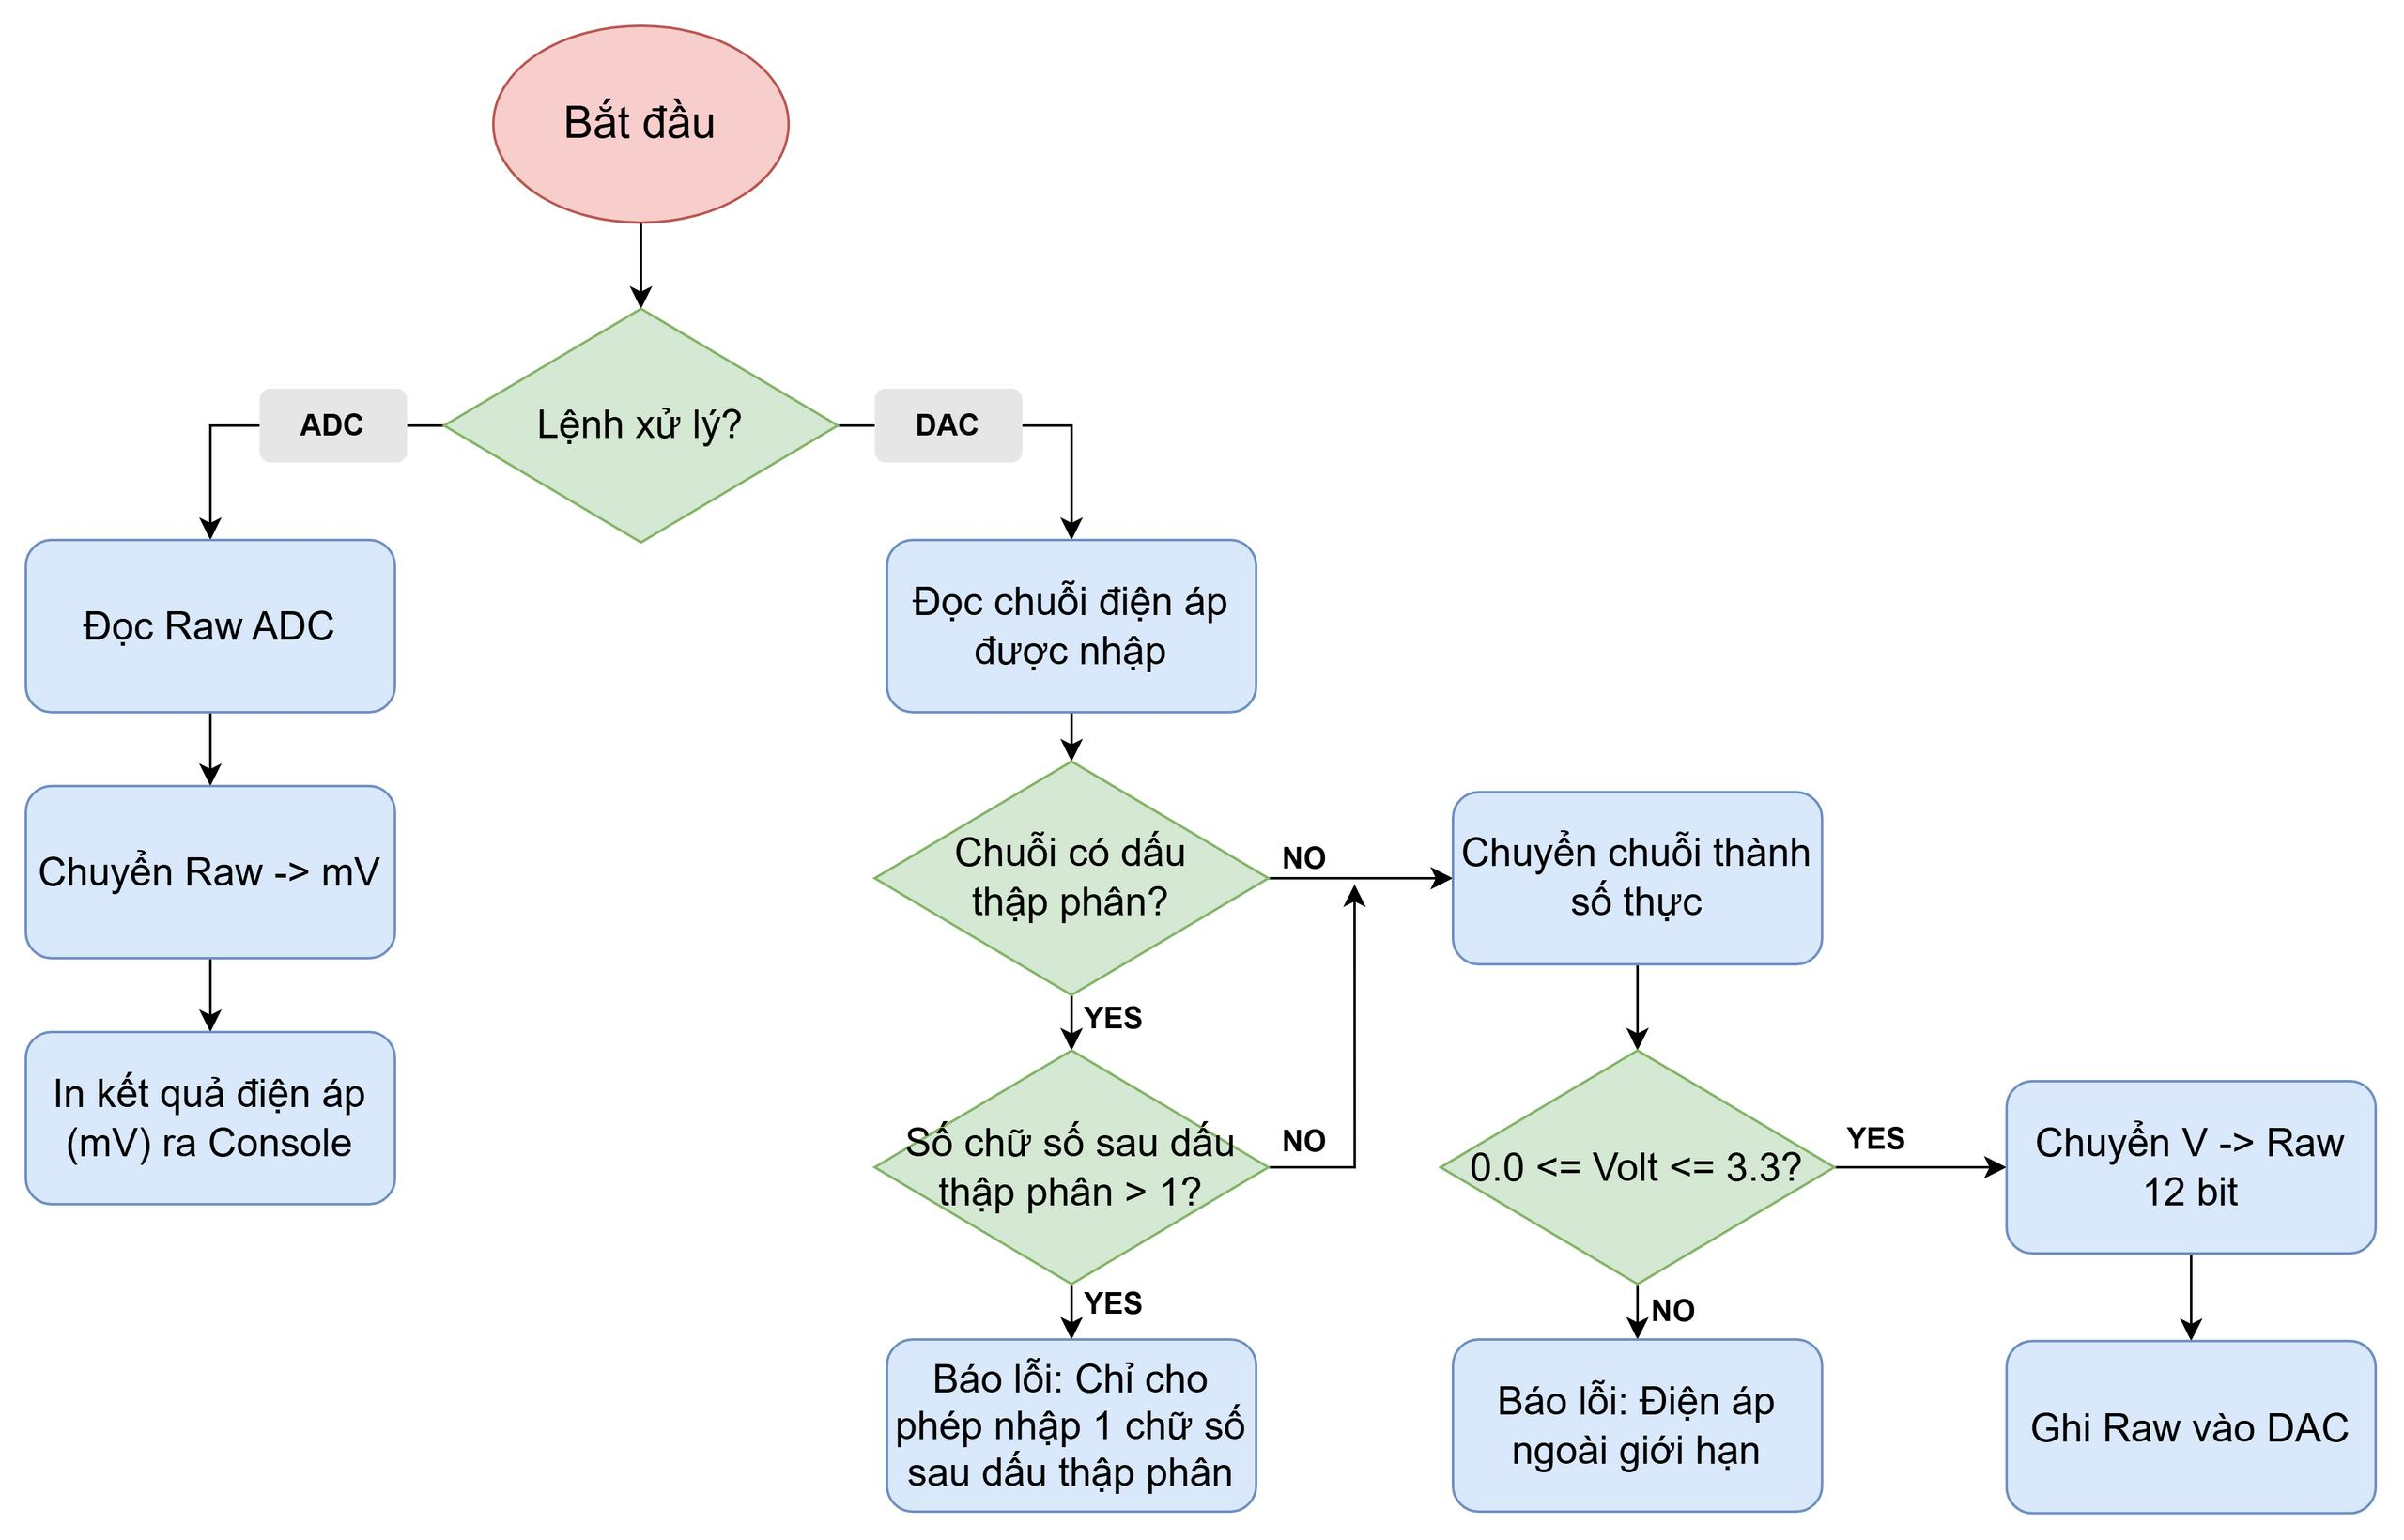
\includegraphics[width=1\textwidth]{image/hil_adc_dac.jpg}
    \caption{Lưu đồ giải thuật xử lý ADC và DAC}
    \label{fig:hil_adc_dac}
\end{figure}
Lưu đồ mô tả giải thuật xử lý cho ADC và DAC. Khi nhận được lệnh đọc ADC, HIL sẽ thu thập giá trị Raw 12 bit từ ADC. Giá trị này được chuyển đổi sang mức điện áp $mV$ theo công thức: $V_{mV}=\dfrac{Raw \cdot 3.3}{2^{12}-1} \cdot 1000$ và tiến hành in kết quả lên Console.

Đối với lệnh cấu hình mức điện áp cho DAC, hệ thống sẽ nhận giá trị điện áp mong muốn dưới dạng một chuỗi ký tự.
Ở bước đầu sẽ kiểm tra trong chuỗi có dấu thập phân hay không. Nếu có thì cần phải đảm bảo sau dấu thập phân chỉ có 1 chữ số.
Sau đó chuỗi sẽ được chuyển thành số thực và tiếp tục kiểm tra giá trị điện áp có nằm trong dải điện áp an toàn của phần cứng từ 0.0V đến 3.3V không.
Khi có các vi phạm trong quá trình kiểm tra trên, hệ thống sẽ không thực thi và in ra thông báo lỗi. Khi mức điện áp đầu vào được xác nhận là hoàn toàn hợp lệ, thuật toán sẽ áp dụng phương trình chuyển đổi ngược $Raw_{DAC} = \dfrac{V_{input}}{3.3} \cdot 4095$ để ánh xạ mức điện áp thành một giá trị nguyên 12 bit tương ứng.
Cuối cùng, giá trị này được ghi vào DAC và xuất tín hiệu điện áp.

\subsection{Tạo sóng sin / sóng tam giác}
Về bản chất, tín hiệu Analog là tín hiệu liên tục theo thời gian và có thể được biểu diễn bởi các mức điện áp thay đổi liên tục.
Để có thể tái tạo tín hiệu Analog bằng hệ thống số, tín hiệu sẽ được cập nhật thành nhiều giá trị điện áp rời rạc tại các thời điểm khác nhau. Nếu khoảng thời gian giữa các lần cập nhật càng nhỏ, hay nói cách khác tần số lấy mẫu càng cao, thì tín hiệu tạo ra sẽ càng tiệm cận với dạng sóng Analog ban đầu và trở nên mượt hơn.
Tần số thực hiện các lần cập nhật này được gọi là tần số lấy mẫu ($f_{sample}$).
\begin{figure}[H]
    \centering
    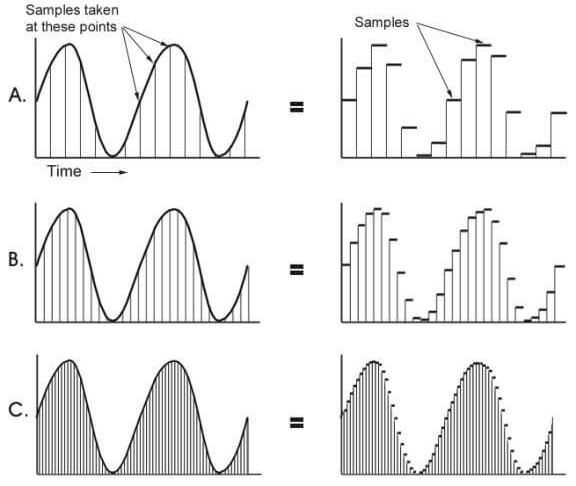
\includegraphics[width=0.6\textwidth]{image/hil_wave_sample.jpg}
    \caption{Quá trình lấy mẫu để tái tạo tín hiệu analog}
    \label{fig:hil_can}
\end{figure}

Từ lý thuyết trên, HIL sẽ thực hiện chức năng tạo sóng sin / tam giác thông qua việc kết hợp DAC, DMA và Timer để tối ưu hóa hiệu suất và đảm bảo tính thời gian thực.
Tần số của Timer ($f_{sample}$) sẽ kích hoạt sự kiện để DMA lấy 1 giá trị trong mảng vùng nhớ để nạp vào DAC và để tạo nên một chu kỳ sóng hoàn chỉnh ta cần $N$ mẫu.
Từ đó ta có thể tính được tần số của sóng như sau:
\begin{equation}
    f_{wave} = \dfrac{f_{sample}}{N}
    \label{eq:f_wave}
\end{equation}

Để tạo được dạng sóng đủ mượt mà không làm giảm quá nhiều tần số của sóng, chọn $N=100$. Với $f_{sample_{max}}$ của hệ thống là 1 $MHz$, tần số tối đa của sóng là 10$kHz$.

\begin{figure}[H]
    \centering
    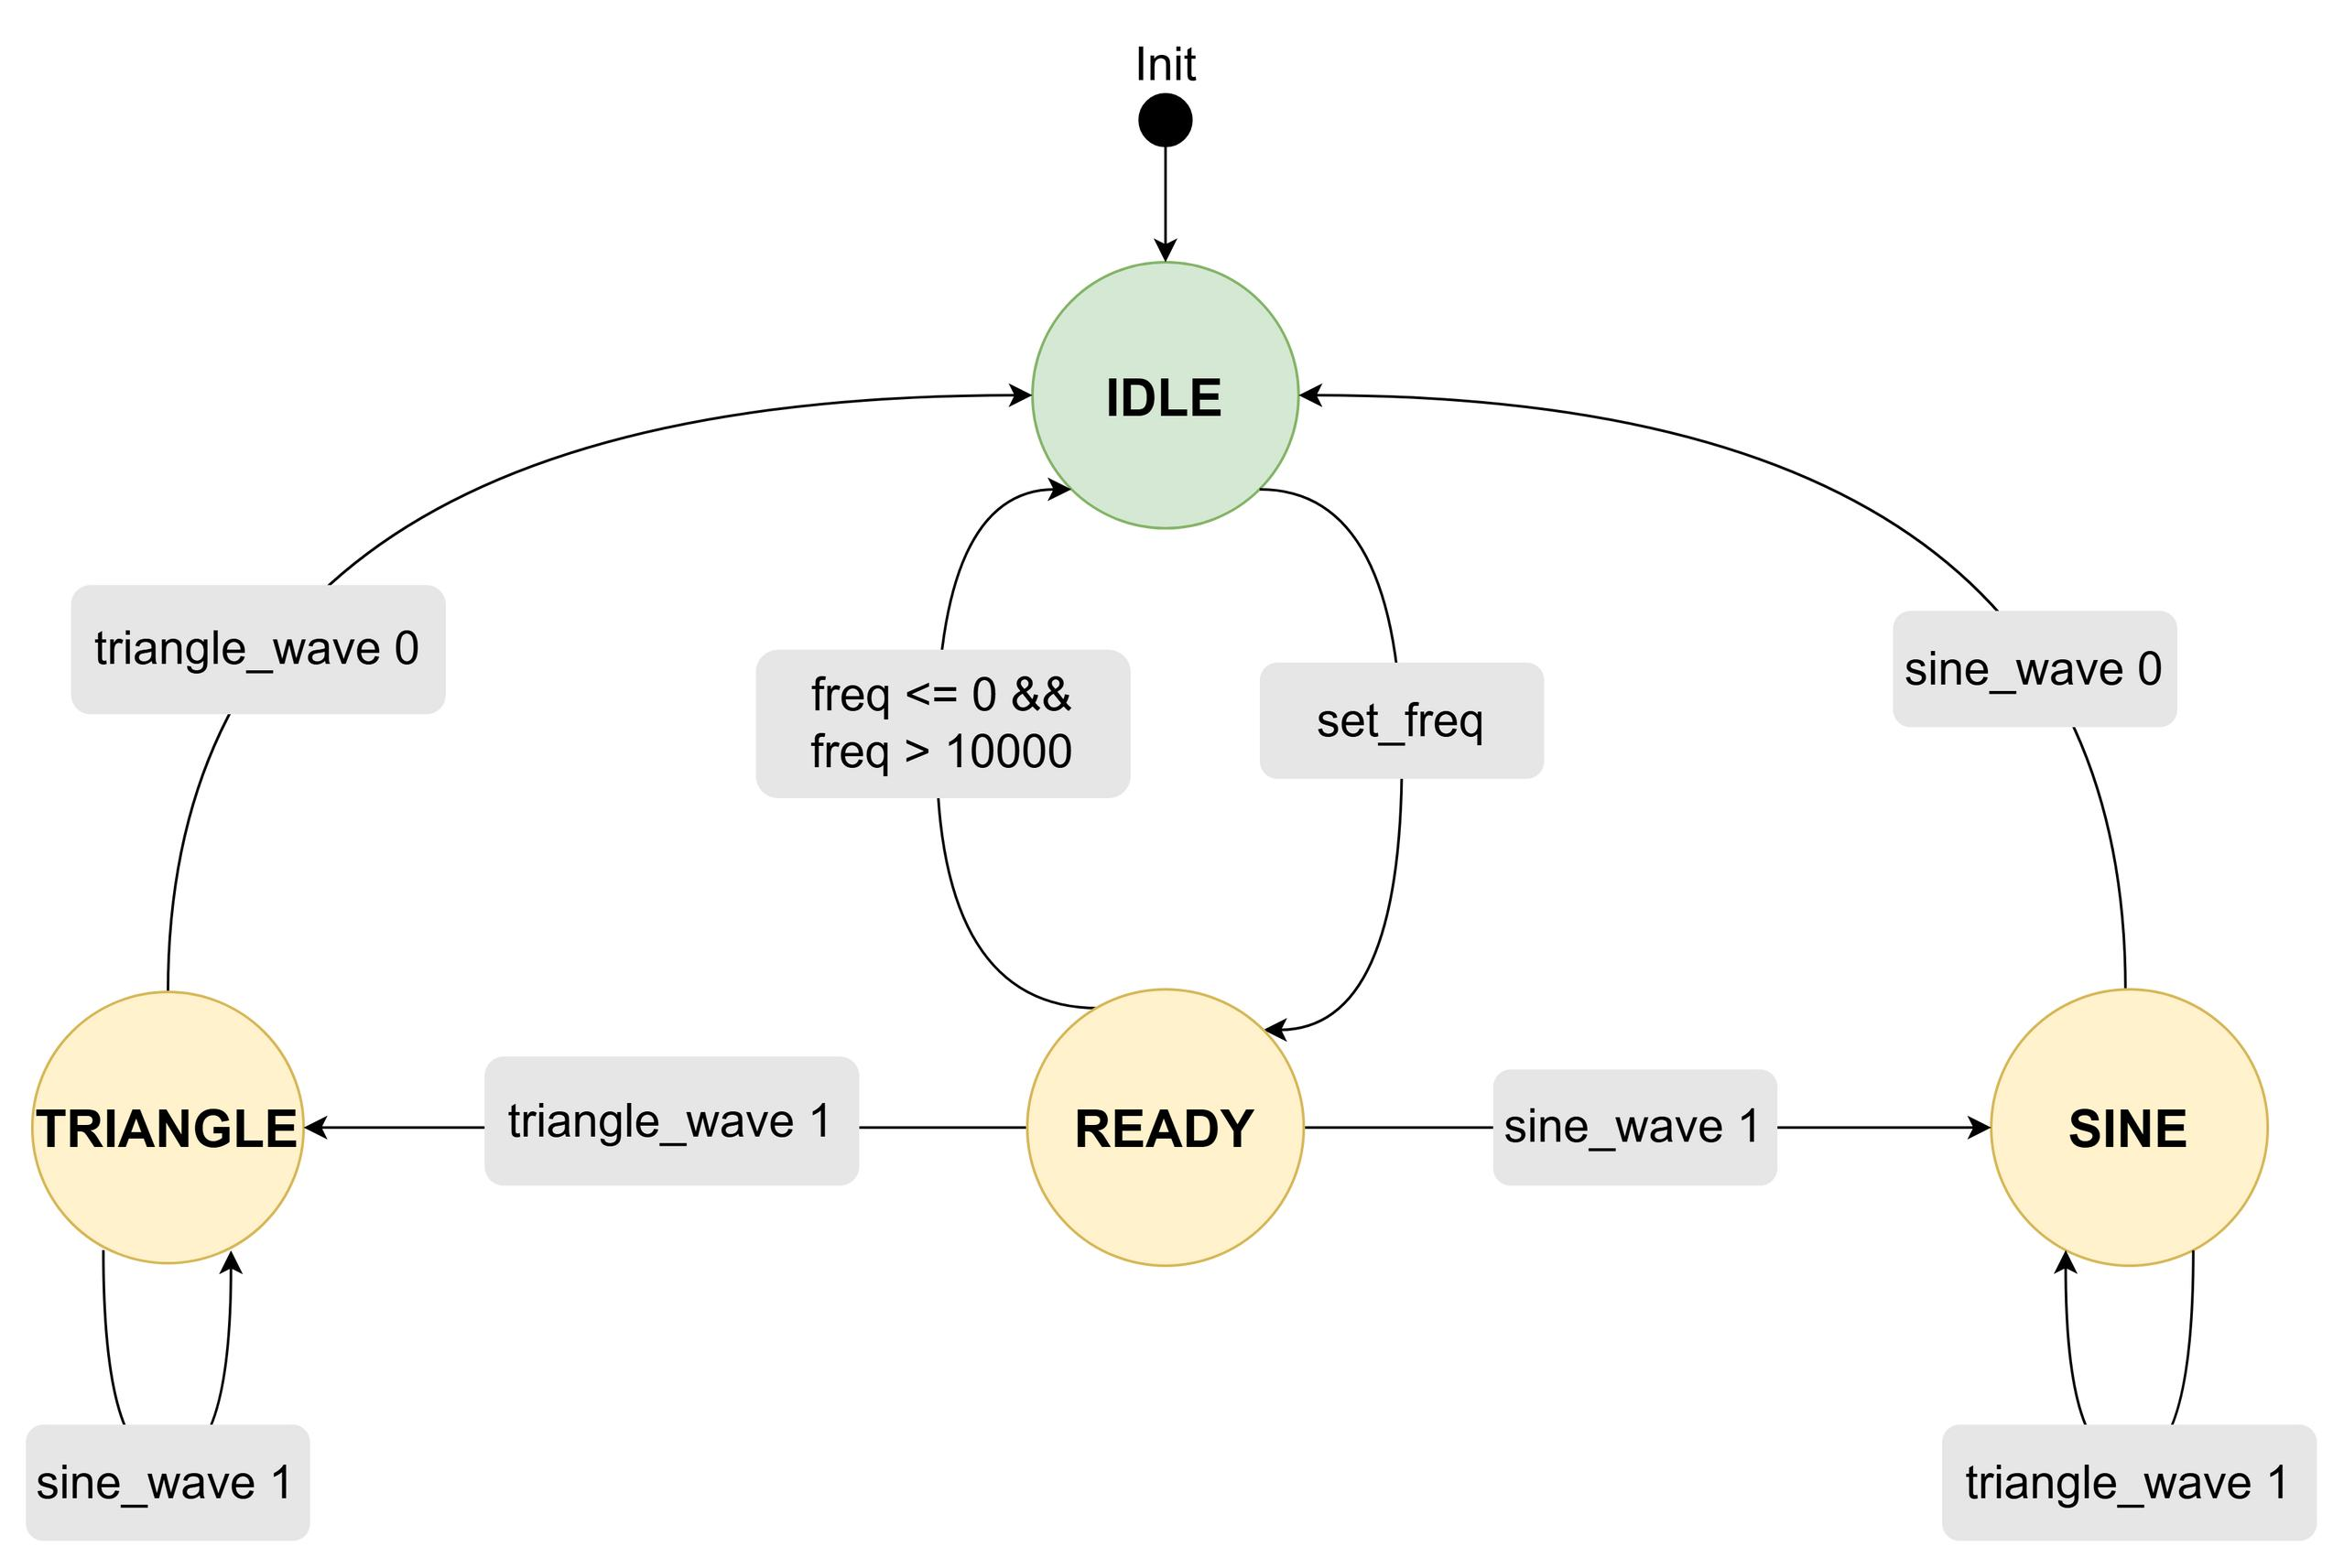
\includegraphics[width=0.8\textwidth]{image/hil_wave.jpg}
    \caption{Sơ đồ máy trạng thái của chức năng tạo sóng}
    \label{fig:hil_wave}
\end{figure}
Chức năng tạo sóng được thiết kế theo sơ đồ máy trạng thái trên với 4 trạng thái chính: \texttt{IDLE} (chờ lệnh cài đặt tần số), \texttt{READY} (chờ lệnh tạo sóng), \texttt{\texttt{SINE}} (tạo sóng sin), \texttt{TRIANGLE} (tạo sóng tam giác).

HIL sẽ cấu hình các ngoại vi cần thiết để thực hiện việc tạo sóng. Trong giai đoạn này, HIL cũng sẽ khởi tạo 2 buffer cho sóng sin và sóng tam giác với số lượng 100 mẫu cho mỗi buffer, công thức cho mỗi dạng sóng sẽ được tính toán ở phần dưới.
Sau giai đoạn khởi tạo, hệ thống sẽ vào trạng thái \texttt{IDLE} để chờ lệnh cấu hình tần số. Khi tần số được cấu hình hợp lệ ($0 < freq \le 10000$), hệ thống chuyển sang trạng thái \texttt{READY} và tính toán tần số cho Timer.
Khi người dùng gửi lệnh bắt đầu tạo sóng sin / tam giác, hệ thống sẽ chuyển sang trạng thái \texttt{SINE} / \texttt{TRIANGLE} tương ứng và bắt đầu tạo sóng. Vì chức năng tạo sóng chỉ được thực hiện bởi 1 phần cứng DAC (PA4) nên tại một thời điểm chỉ có thể tạo được 1 dạng sóng.
Cơ chế này giúp bảo vệ phần cứng không bị xung đột. Cuối cùng, khi có lệnh dừng việc tạo sóng, HIL sẽ trở về trạng thái \texttt{IDLE}.

DAC của STM32F407 có độ phân giải 12 bit, nên giá trị tối đa ($DAC\_MAX$) có thể xuất ra là $2^{12} - 1 = 4095$, tương ứng với mức điện áp 3.3V.

\textbf{Công thức tính toán cho các dạng sóng:}

Đối với sóng sin, biên độ của từng mẫu thứ $i$ (với $i$ chạy từ 0 đến $N-1$) được tính bằng hàm lượng giác và cộng thêm offset để đảm bảo giá trị luôn dương.
\begin{equation}
    V_{sine}[i] = \left( \sin\left(\dfrac{i \cdot 2\pi}{N}\right) + 1 \right) \cdot \dfrac{DAC\_MAX}{2} \cdot 0.98
\end{equation}
Trong đó, hệ số 0.98 được thêm vào nhằm giảm biên độ cực đại chống hiện tượng xén đỉnh.

Đối với sóng tam giác, chu kỳ sóng được chia làm hai nửa đối xứng để tạo độ dốc tuyến tính.
\begin{itemize}
    \item Ở nửa chu kỳ tăng đầu tiên ($i < \dfrac{N}{2}$):
    \begin{equation}
        V_{triangle}[i] = \dfrac{2 \cdot DAC\_MAX \cdot i}{N}
    \end{equation}
    \item Ở nửa chu kỳ giảm tiếp theo ($i \ge \dfrac{N}{2}$):
    \begin{equation}
        V_{triangle}[i] = \dfrac{2 \cdot DAC\_MAX \cdot (N - i)}{N}
    \end{equation}
\end{itemize}

\subsection{Tạo tín hiệu PWM}

\subsection{Xử lý GPIO}
